\documentclass[french]{standalone}
\usepackage{babel}
\usepackage{tkz-fct}
\usepackage{tkz-euclide}
\usepackage{color}
\usepackage{numprint}
\renewcommand*\familydefault{\sfdefault}
\usepackage{sansmath}
\sansmath
\definecolor{gray75}{gray}{0.75}

\begin{document}
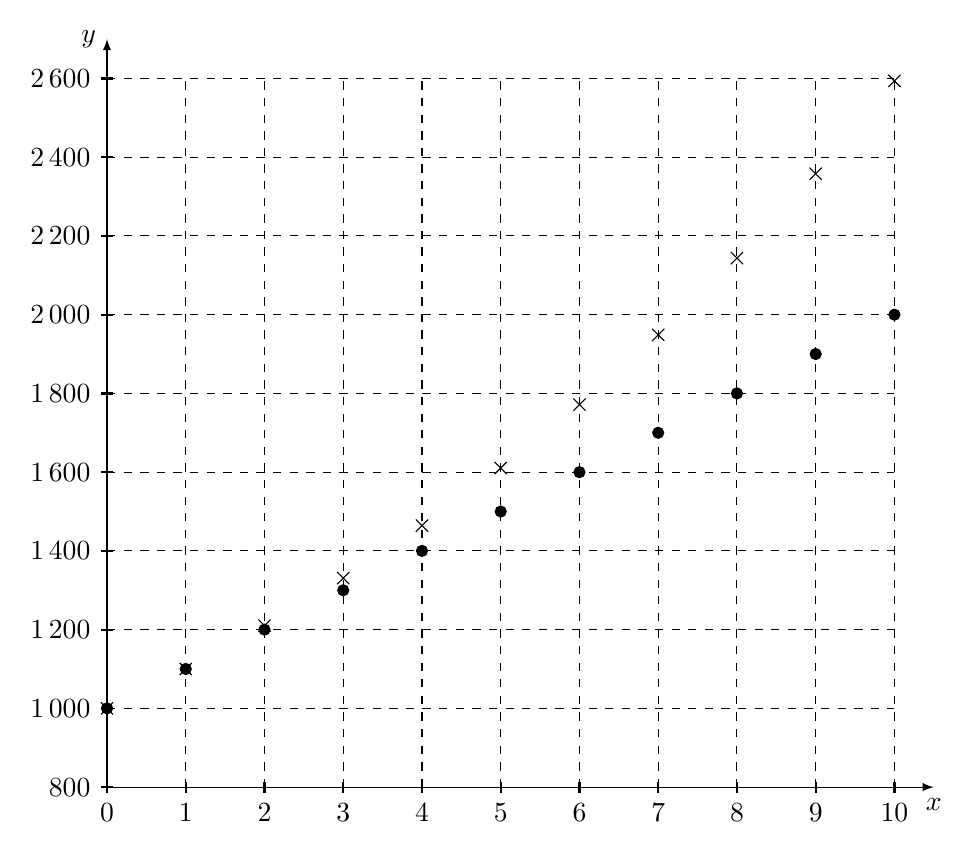
\begin{tikzpicture}
\tkzInit[xmin=0,xmax=10,ymin=800,ymax=2600, ystep=200]
\tkzAxeXY
  \begin{scope}[dashed]
     \tkzGrid[color=black]
   \end{scope}
\tkzSetUpPoint[size = 4]
\global\edef\tkzFctLast{1000*(1+0.1*x)}
\foreach \va in {0,...,10}{%
  \tkzDefPointByFct[draw](\va)
}
\tkzSetUpPoint[shape=cross out,size=4]
\global\edef\tkzFctLast{(1000*exp(x*ln(1.1)))}
\foreach \va in {0,...,10}{%
  \tkzDefPointByFct[draw](\va)
}

\end{tikzpicture}
\end{document}
